\subsubsection{Comparing Data Sets and Files}
Comparing data sets is maybe the most important feature of this service. In doing this, a researcher can evaluate index values over time, using different data sets for different things. For example, a researcher may be working in a site, recording data in the morning and at night, every day for a week. The researcher would process both sets separately using whichever indices and parameters they wish, and name and tag the sets appropriately. Then, in the Catalog, they can select both data sets, and see visualizations comparing the two sets across time, to see how the index values match up on the same days but in the morning and at night.\par
From a research perspective, this is the best way to draw conclusions from the indices included in this service, as the more data that is collected and processed, the more sense they make. An example of this includes a forest where human interaction is on the rise. Using an index like ACI over time will help to make correlations as to how human invasion on the forest is affecting the wildlife. Alternatively, for comparing across sites, if a species of animal is found in multiple locations, the ACI index can be used to roughly determine the number of these species in the area. Comparing this value across the sites is useful for determining species population in different areas.\\

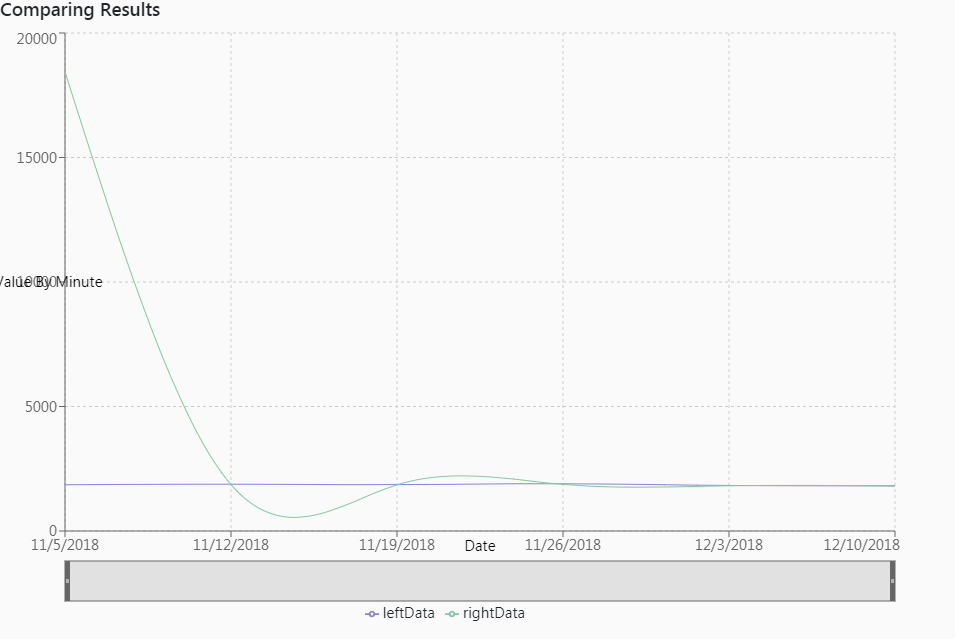
\includegraphics[width=\textwidth]{CompareACIgraph1}\\
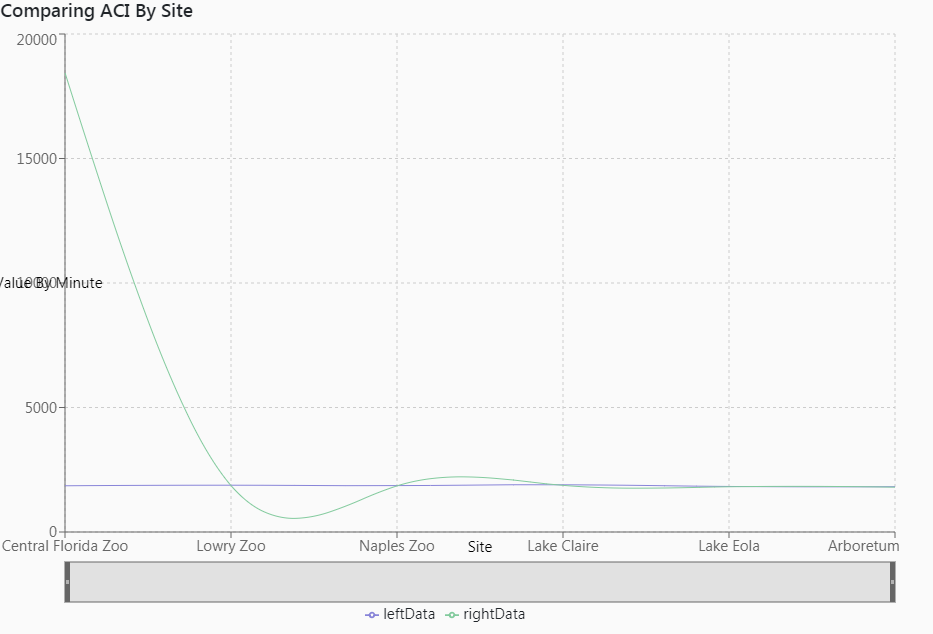
\includegraphics[width=\textwidth]{CompareACIgraph2}\\
The first is a comparison graphic for ACI index across time. The data used was six files, all recorded a week apart. The X axis represents the date of each file, and the Y axis shows the ACI value by minute for each date. The other comparison available for ACI is comparing across data sites. Much like the other ACI comparison graph, the Y axis again shows the ACI value by minute, while the X axis for this graph represents the site. Overall, these two comparison charts give the researcher two different comparison insights for the ACI index.\\

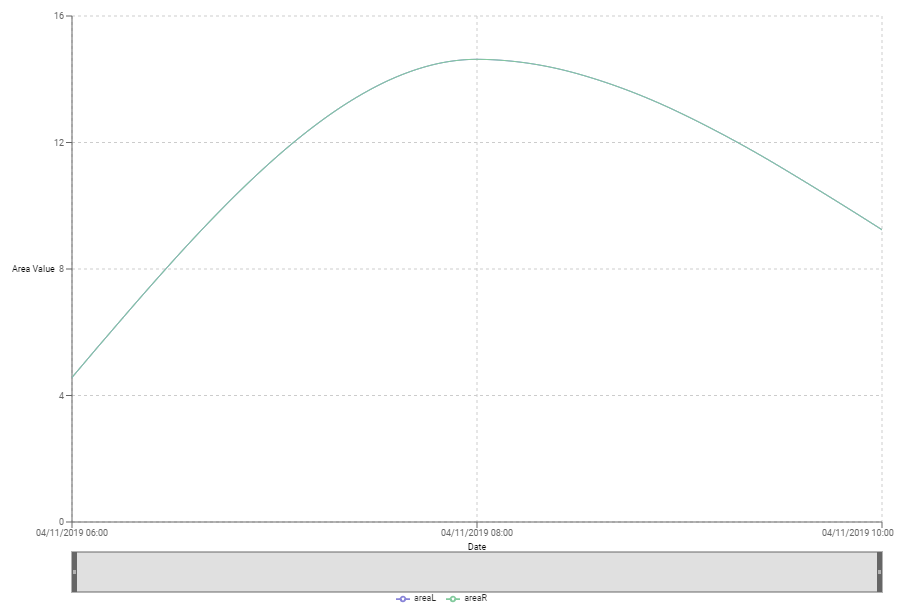
\includegraphics[width=\textwidth]{CompareBAgraph1}\\
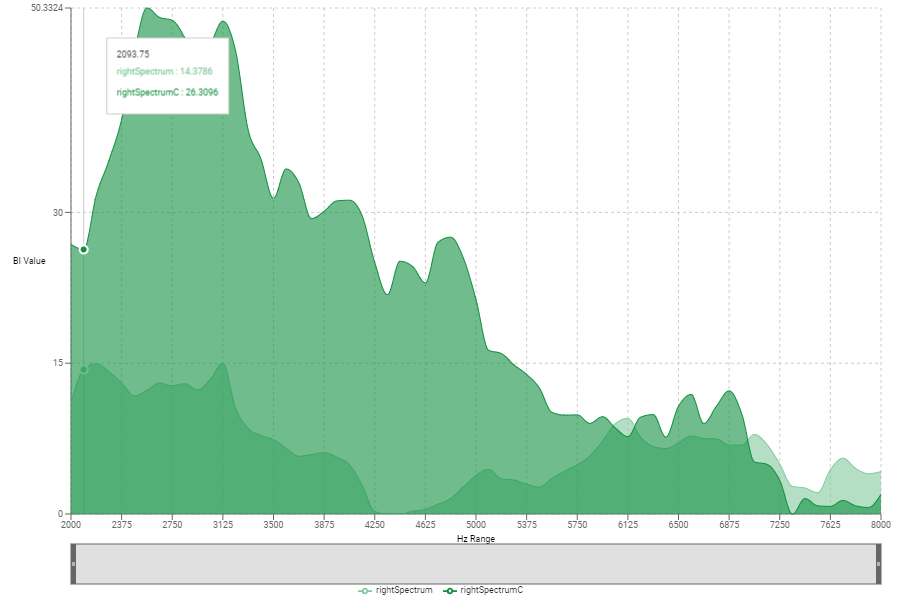
\includegraphics[width=\textwidth]{CompareBAgraph2}\\
These two graphs represent the comparison charts available for the Bioacoustic Index. Again, the user has comparison across dates and research sites available to them. The brush is included to allow the user to shorten the observed time range as they please.\\

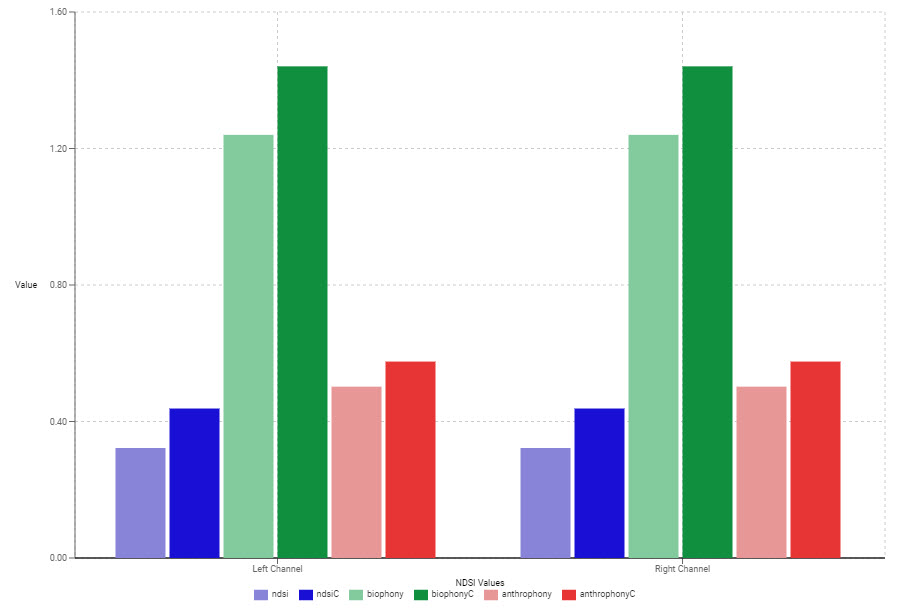
\includegraphics[width=\textwidth]{CompareNDSIgraph1}\\
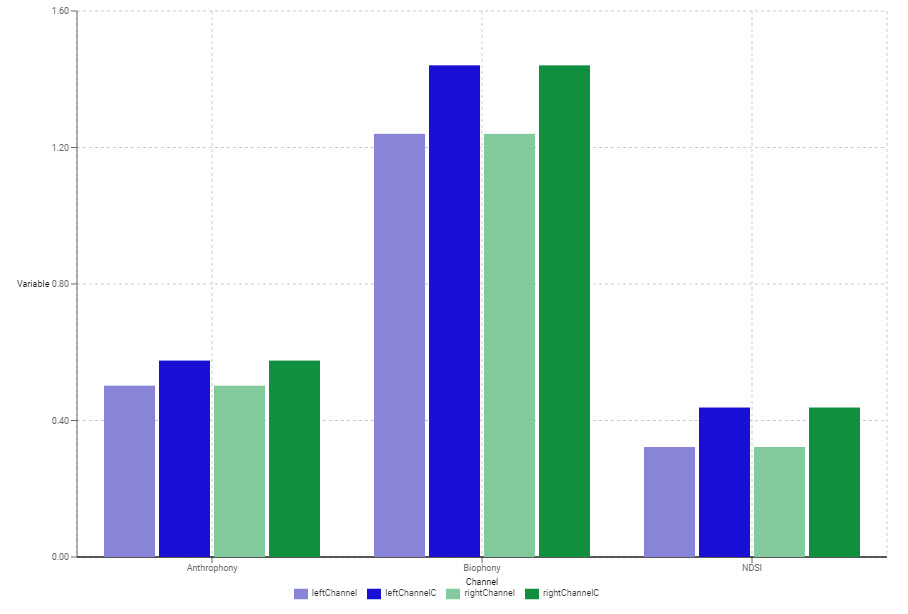
\includegraphics[width=\textwidth]{CompareNDSIgraph2}\\
The NDSI index includes three different variables of interest to the user. These two images show the biophony comparison across date and the NDSI comparison across sites respectively. These charts are bar graphs to show the respective value by channel, along with a line that helps to show the change intensity between values. Notice that the NDSI is upside down, this is because NDSI values are typically negative due to the nature of the index. A brush is included as per usual.\\
